\documentclass[12pt]{article}
\usepackage[T1]{fontenc} 
\usepackage[icelandic]{babel}
\usepackage{latexsym,amssymb,amsmath}
\usepackage{graphicx}
\usepackage{hyperref}
\usepackage{enumerate}
\usepackage[most]{tcolorbox}
\usepackage{pgfplots}
\usepackage{nicefrac}
\usepackage{derivative}
\usepackage{setspace}
\usepackage{caption}
\usepackage{subcaption}

\pgfplotsset{compat=1.17}
\voffset=-1.0in
\hoffset=-0.5in
\textwidth=6in
\textheight=9.0in
\setlength{\jot}{.8em}
\captionsetup{labelfont=bf}

%\renewcommand{\rmdefault}{\sfdefault}
\onehalfspacing

\title{\bfseries Hermilíkanið TEST}
\author{Kári Hlynsson \vspace*{2mm} \\ \small Erfðafræði, Menntaskólanum í Reykjavík \\ \small Kennari: Andri Guðmundsson}
\date{}

\begin{document}

\maketitle

\begin{abstract}
    \noindent
    Kynnt er TEST hermilíkanið (\emph{Temporal Evolutionary Simulation Tool}) sem hermir
    aðlögun náttúrulegs þýðis að umhverfi sínu sem afleiðing náttúruvals. Við könnum
    samband milli umhverfisþáttar $\varphi$ og meðalhæfni $\omega_{\mathrm{avg}}$ og sýnum að
    þegar enginn umhverfisþáttur er til staðar er ekki stefnd breyting á meðalhæfni. Fræðileg
    undirstaða er tekin fyrir og niðurstöður hermunar raktar. Greinin er ítarefni á fyrirlestri
    sem var kynntur í erfðafræðiáfanga við Menntaskólann í Reykjavík.
\end{abstract}

\section{Fræðileg undirstaða}
Ein af meginkenningum Charles Darwin eru þær að tilhneiging náttúrulegs þýðis sé sú að einstaklingar
sem eru betur aðlagaðir umhverfi sínu eru líklegri til að fjölga sér og bera þannig erfðir sínar áfram.
Efni fyrirlestursins og þessa skýrslu er að kanna einmitt þessa kenningu en þetta skal gert með hermun (e. \emph{simulation}).
\par Við notum stærðfræðilegan rithátt til að einfalda framsetningu. $P = \{i_1, \ldots, i_n\}$ táknar náttúrulega þýðið sem er til skoðunar, sem samanstendur
af $N$ einstaklingum. Hæfni einstaklings er táknuð $\omega_i$ þar sem $i$ er einstaklingurinn. Jafnframt er $\omega_{\mathrm{avg}}$ meðalhæfni
þýðisins $P$ og er reiknuð
\[
    \omega_{\mathrm{avg}} = \frac 1N \sum_{i = 1}^N \omega_i
\]
Umhverfisþátturinn $\varphi \in \mathbb R^+$ er það sem við notum til að kanna hvort einstaklingur lifi af einhvern erfiðleika í umhverfinu
sem betur aðlagaðir einstaklingar eiga auðveldar með að lifa af. Yrðingin $\hat S(i)$ er \emph{afkoma einstaklings} $i$ og er skilgreind
\[
    \hat S(i) = \omega_i \geq \varphi
\]
Ef fyrir einstakling $i$ gildir $\lnot \hat S(i)$ þá deyr einstaklingurinn en annars ekki. Þetta er bara ef einstaklingurinn er
útsettur fyrir umhverfisþættinum, sem við skoðum hér fyrir neðan.
\par Talan $\lambda \in [0;1]$ er hlutfall þýðisins sem er útsettir fyrir umhverfisþættinum á hverri tímaeiningu. Við höfum því að
$N_\lambda = \lambda N$ þar sem $N_\lambda$ táknar fjölda einstaklinga sem eru útsettir. Þeir eru valdir úr þýðinu með slembnu ferli.
\par Líkanið tekur inn stika $\Delta \varphi$ sem er þannig að á hverri tímaeiningu hækkar gildi umhverfisþáttar $\varphi$ um einmitt þessa
stærð, þ.e. $\frac{\mathrm d \varphi}{\mathrm dt} = \Delta \varphi$ þ.a. $\varphi_{t + 1} = \varphi_t + \Delta \varphi$.
\par Þeir einstaklingar sem lifa af umhverfisþáttinn (eða eru ekki útsettir fyrir honum) fjölga sér (eru afritaðir inn í þýðið) og hæfni afkvæmisins fæst
af slembnu reikniferli $R(\omega_i)$:
\[
    R(\omega_i) = \begin{cases}
        \omega_i + \Delta \omega   & \text{fyrir $\textbf{Unf}[0;1] < \tau$} \\
        \omega_i - \Delta \omega   & \text{fyrir $\textbf{Unf}[0;1] > 1 - \tau$} \\
        \omega                     & \text{annars.}
    \end{cases}
\]
en hér er $\textbf{Unf}$ jafna líkindadreifingin yfir bilið $[a;b]$ þannig að $\mathrm{Pr}\{X = x\} = \frac{1}{b - a}$ þar sem $x \in [a;b]$. Stærðin
$\Delta \omega$ fylgir einnig jafnri líkindadreifingu nema yfir bilið $[0;0.3]$ og segir til um hve mikið hæfni afkvæmisins getur breyst af völdum
skaðlegrar/hagstæðrar stökkbreytingar. Í líkaninu notum við $\tau = 0.025$ þó því megi breyta eftir vilja.
\section{Markmið}
\noindent Markmiðið er að sýna að $\omega_{\mathrm{avg}} \propto \varphi$. Með öðrum orðum viljum við sýna að þýðið aðlagist umhverfisþætti sínum.
Þetta segir okkur að samfelld aukning í meðalhæfni þýðis er afleiðing umhverfisþáttar. Þetta gefur þess auki til kynna að ef enginn umhverfisþáttur
er til staðar í umhverfinu eða $\varphi \ll \omega_{\mathrm{avg}}$, þá búumst við ekki við miklum breytingum á meðalhæfni. Setjum þannig fram eftirfarandi tilgátur:
\begin{enumerate}
    \item[(1)] Ef $\omega_{\mathrm{avg}} \sim \varphi$ í upphafi hermunar, þá er vaxandi samband milli
    $\omega_{\mathrm{avg}}$ og $\varphi$.
    \item[(2)] Ef $\omega_{\mathrm{avg}} \gg \varphi$ eða $\varphi = 0$, þá er engin markviss breyting á meðalhæfni í þýðinu.
\end{enumerate}

\section{Aðferðafræði}
Líkanið flytur gögn yfir á CSV (e. \emph{comma separated values}) snið sem við notum til tölulegrar úrvinnslu.
Öll töluleg úrvinnsla var gerð í RStudio en þess auki teiknar líkanið mynd af hermuninni sem má sjá á mynd \ref{fig:simulation}.

\begin{figure}[ht!]
    \centering
    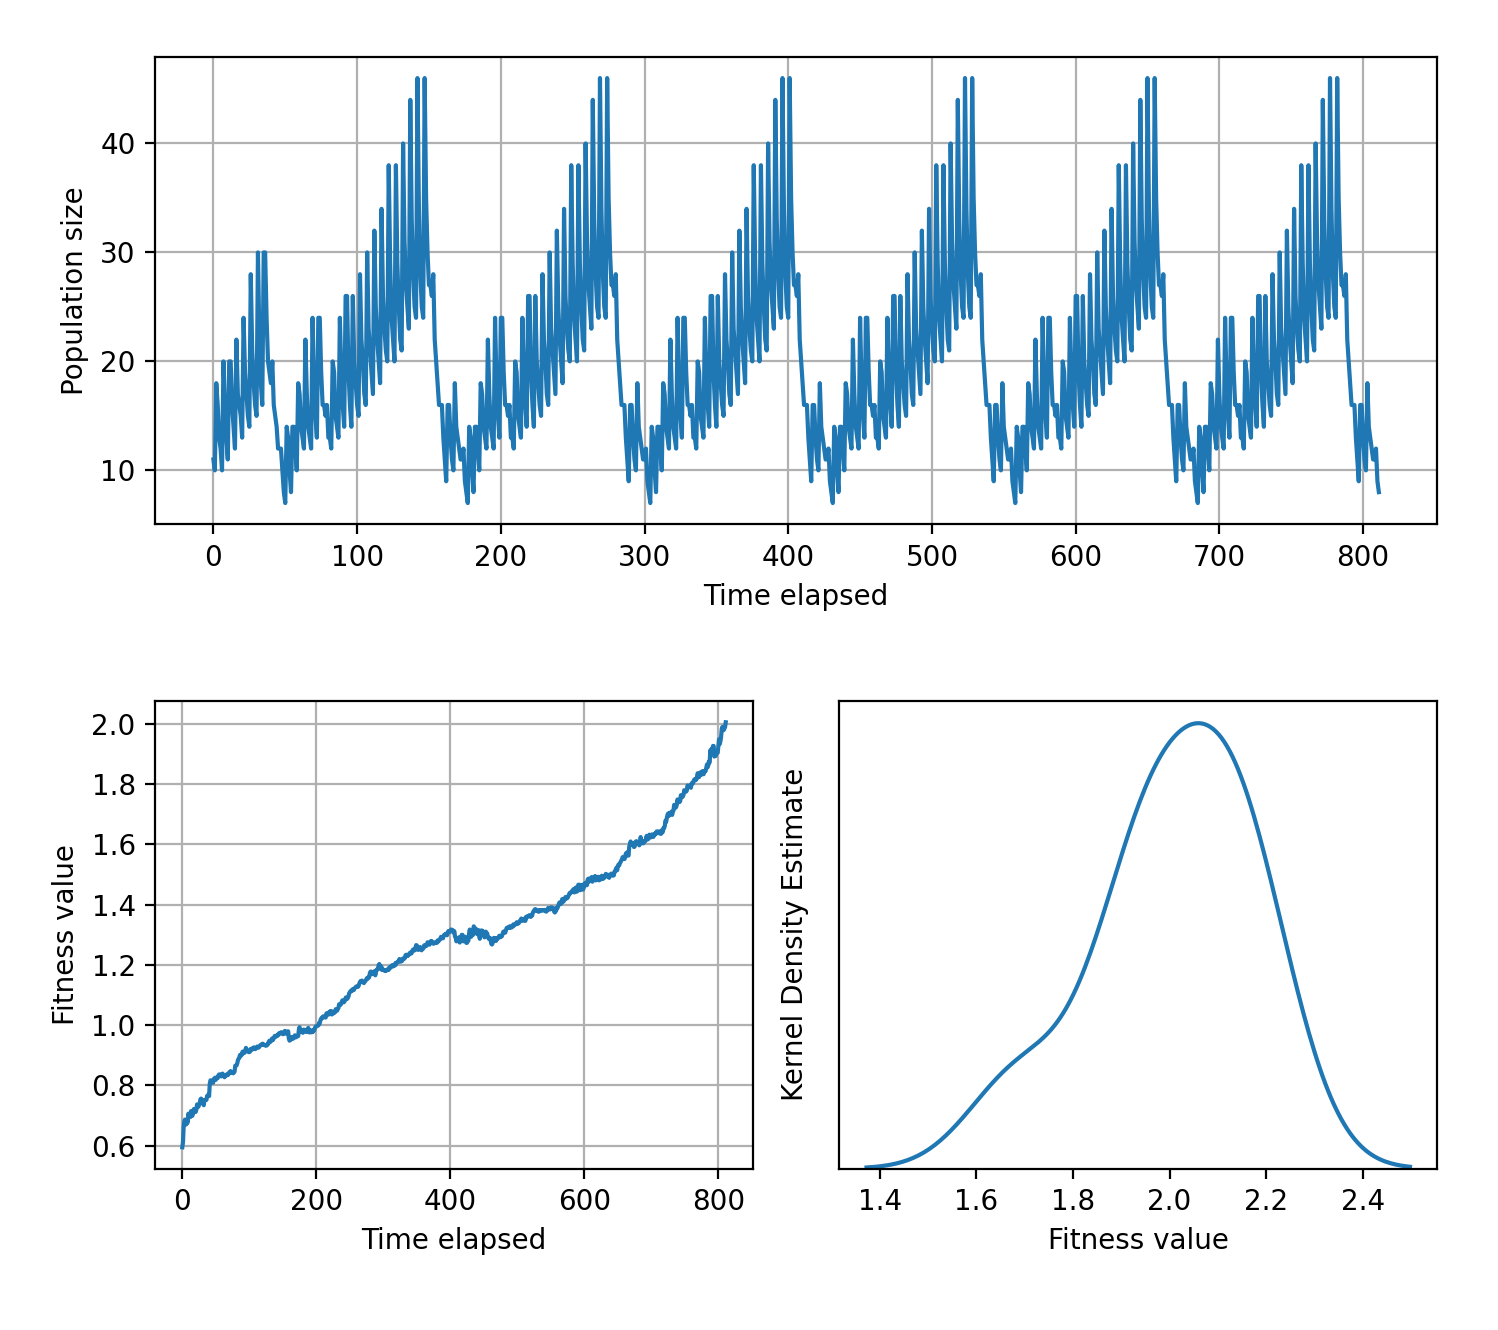
\includegraphics[width=0.8\textwidth]{img/sim_visualization.png}
    \caption{Myndrænn þáttur líkansins} \label{fig:simulation}
\end{figure}

Látum $\mathbf x = \{x_1, \ldots, x_n\}$ og $\mathbf y = \{y_1, \ldots, y_n\}$ vera $n$ mælingar á slembistærðum $X$ og $Y$. Meðaltöl úrtakanna 
ritum við $\overline x$ og $\overline y$ en staðalfrávik þeirra $s_x$ og $s_y$. Fylgnistuðullinn er sú stærð sem lýsir sambandi breytanna tveggja
og er skilgreind
\[
    \rho = \frac{1}{n - 1} \sum_{i = 1}^n \left(\frac{x_i - \overline x}{s_x}\right)\left(\frac{y_i - \overline y}{s_y}\right)
\]
Fylgnistuðullinn er alltaf á bilinu $[-1;1]$. $\rho > 0$ gefur til kynna jákvæða fylgni (vaxandi samband) en $\rho < 0$ neikvæða fylgni (minnkandi samband). Tilgátur (1) og (2) má því endurorða út frá gildinu á $\rho$, þ.e. hvort það sé jákvætt, neikvætt eða núll.

\section{Niðurstöður}
\subsection{Gildi umhverfisþáttar lágt eða núll}
Skoðum tilfelli þar sem $\varphi = 0$ með engri aukningu í umhverfisþætti. Í $t = 0$ er $n = 10$. Mynd af meðalhæfni $\omega_{\text{avg}}$
sem fall af tíma $t$ má sjá á mynd 2. Línulegt aðhvarf á þessari hermun gaf $R^2 = 0.1838$ sem segir okkur að breytingar á meðalhæfni
er erfitt að skýra út af breytingu á tíma. Við látum það því nægja til að sýna fram á tilgátu (2) um að engin markviss (stefnd) breyting
á meðalhæfni má skýra með breytingu á tíma.
\begin{figure}[ht!]
    \centering
    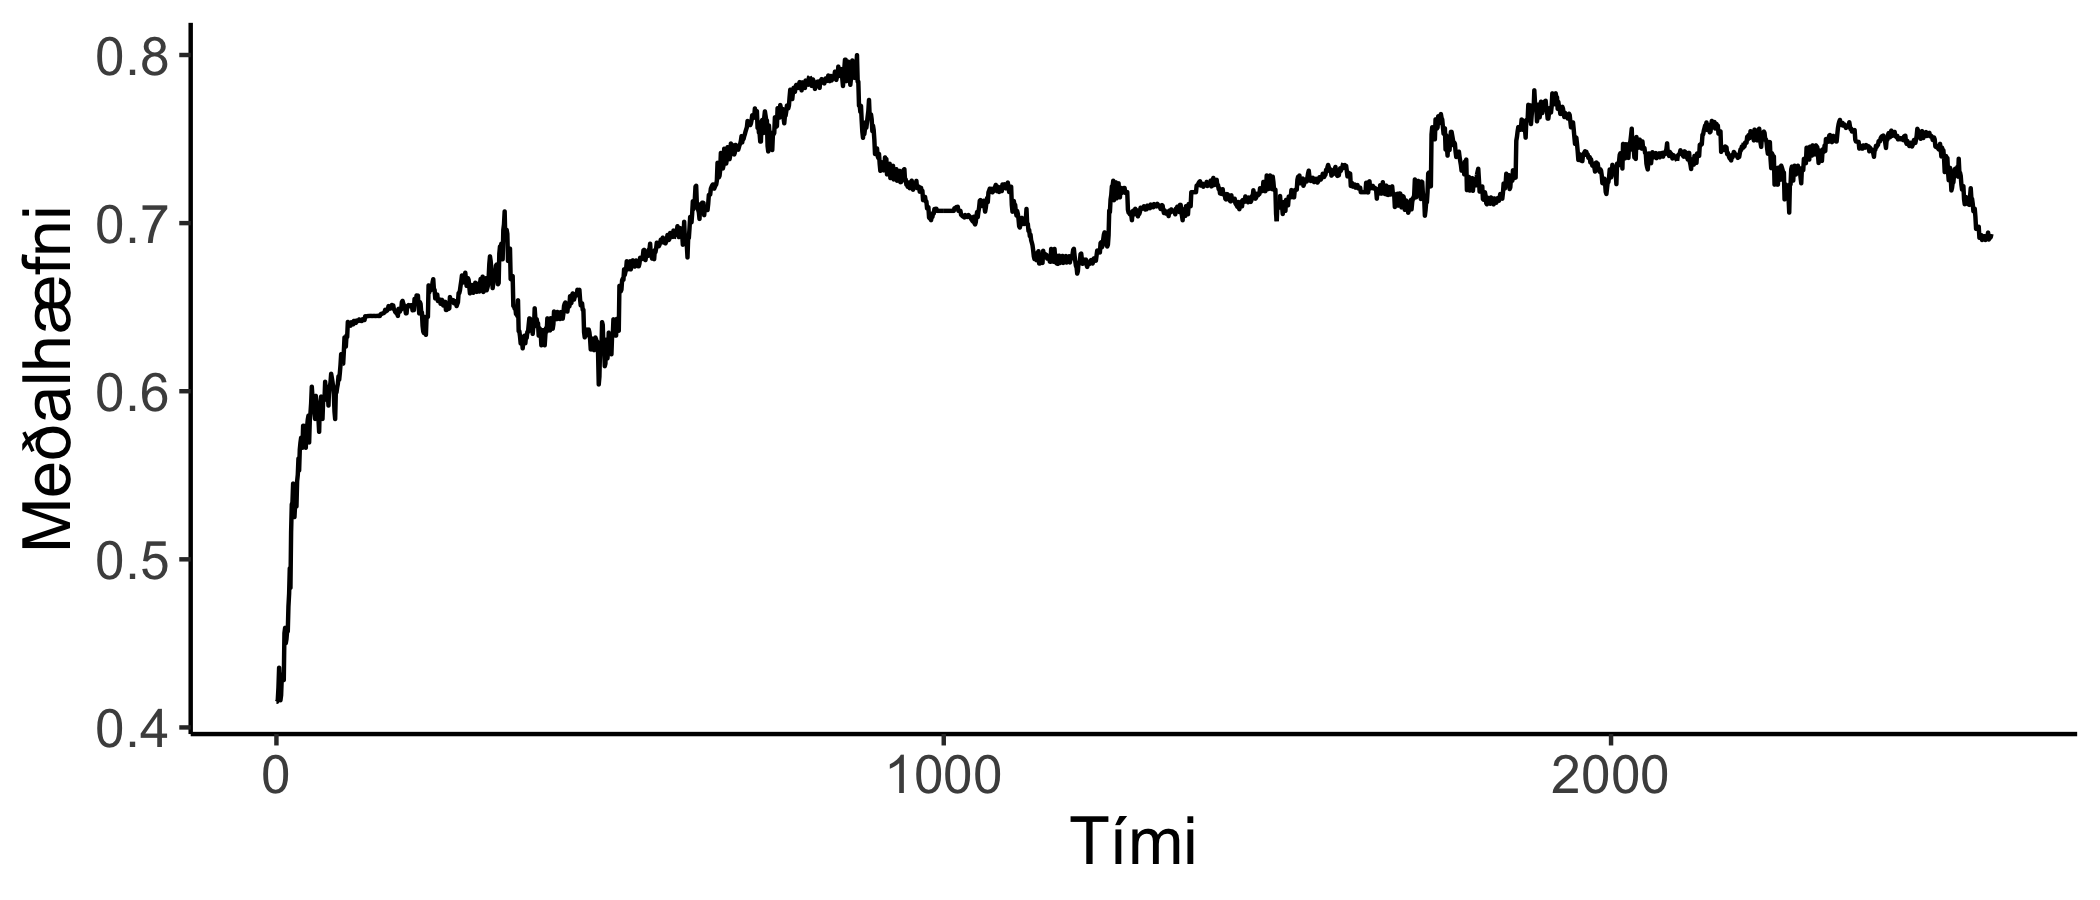
\includegraphics[width=0.85\textwidth]{img/fig-noenv.png}
    \caption{Meðalhæfni yfir tíma í hermun með $\varphi = 0$}
\end{figure}
\par
Það er varasamt að draga þá ályktun að stefnd breyting (þ.e. vaxandi/minnkandi) á meðalhæfni sem fall af tíma sé til marks um hið gagnstæða 
við það sem segir hér að framan. Það er mun frekar að handahófskenndar stökkbreytingar afkvæma leiða af sér hærri eða lægri hæfni sem hefur
auðvitað áhrif á meðaltal þýðisins. Þessir einstaklingar fjölga sér og þannig hækkar meðaltalið til lengri tíma. Skoðum þetta aðeins nánar.
\par
Látum $\{\mu_B\}_{t \geq 0}$ og $\{\mu_D\}_{t \geq 0}$ vera líkindaferlin sem gefa fjölda stökkbreytinga sem hafa orðið. Hér er $\mu_B$ hagstæð stökkbreyting
(e. \emph{beneficial}) en $\mu_D$ skaðleg (e. \emph{detrimental}). Líkindadreifing beggja ferla er tvíkostadreifing (e. \emph{binomial distribution}) sem er strjál líkindadreifing með forskriftina
\[
    \mathrm{Pr}\{\mu_G = k\} = {t \choose k} \tau^k(1 - \tau)^{t - k}
\]
þar sem $\mu_G$ er annað hvort $\mu_B$ eða $\mu_D$. Hér eftir látum við $k$ tákna fjölda hagstæðra stökkbreytinga en $j$ fjölda skaðlegra.
\par Til þess að breyting á meðalhæfni sé strangt stefnd þarf að gilda annaðhvort $j = 0$ eða $k = 0$. Skoðum fyrra tilfellið og látum $(\mu_B)_t^* = k^*$ og $j = 0$
þar sem $t^*$ er tími liðinn í hermuninni fram að þessu.
Úr því að ferlin eru óháð hvor öðrum gildir að líkindi þess að báðir atburðir verða eru jöfn margfeldi líkinda atburðanna beggja hvort um sig, það er að segja
\begin{align*}
   \mathrm{Pr}\{k = k^* \land j = 0\} &= \mathrm{Pr}\{k = k^*\} \mathrm{Pr}\{i = 0\} \\
                               &= {t^* \choose k^*}{t^* \choose 0} \tau^{k^*} \tau^0 (1 - \tau)^{t - k^*} (1 - \tau)^{t - 0} \\
                               &= {t^* \choose k^*}\tau^{k^*} (1 - \tau)^{2t - k^*}
\end{align*}
En við sjáum að $\mathrm{Pr}\{k = k^*, i = 0\} \leq \mathrm{Pr}\{k = k^*, i > 0\}$ fyrir öll gildi á $k^*$ og $i$ svo líkurnar á strangt stefndri
meðalhæfnisbreytingu eru hverfandi litlar. Við látum ótalið að sanna veika tilfellið þar sem $i \neq 0$ eða $k \neq 0$ en annað hvort $i \gg k$ eða
$k \gg i$, en sú umfjöllun sem hefur verið rakin hér að ofan verður látin nægja að sinni.

\subsection{Umhverfisþáttur sem skýribreyta aukinnar meðalhæfni}
Gögnum var safnað með því að keyra líkanið með þeim stikum sem má sjá í töflu fyrir neðan.
Þetta var gert til að sýna hvernig mismunandi gildi breyta hafa áhrif á hvort annað. Reynt
var að hafa $t \approx 2000$.
\renewcommand{\arraystretch}{1.4}
\begin{table}[ht!]
    \centering
    \begin{tabular}{l c c c c|c}
        \hline
        $^\text{\text{(\textasteriskcentered)}}$ Skráarheiti                                & $\varphi$ & $\Delta \varphi$  & $n_{t = 0}$ & $\lambda$ & $\rho_{\omega_{\mathrm{avg}} \sim \varphi}$ \\
        \hline
        $^{\textbf{(A)}}$ \texttt{data-medphi-loDphi-medlambda.csv}  & 0.50      & 0.001             & 10          & 0.10       & 0.7024183  \\
        $^{\textbf{(B)}}$ \texttt{data-medphi-hiDphi-medlambda.csv}  & 0.50      & 0.005             & 10          & 0.10       & 0.6802611  \\
        $^{\textbf{(C)}}$ \texttt{data-hiphi-loDphi-medlambda.csv}   & 1.00      & 0.001             & 10          & 0.10       & -0.8965901 \\
        $^{\textbf{(D)}}$ \texttt{data-hiphi-hiDphi-medlambda.csv}   & 1.00      & 0.005             & 10          & 0.10       & -0.1110411 \\
        \hline
        \footnotesize{$^\text{\text{(\textasteriskcentered)}}$ Merki hermunar á mynd fyrir neðan }
    \end{tabular}
    \caption{Mismunandi gildi breyta notuð við hermanir}
\end{table}

\par
\noindent 
Mynd 3 á næstu síðu sýnir $\omega_{\mathrm{avg}}$ og $\varphi$. Athyglisvert er að ef $\varphi \gg \omega_{\mathrm{avg}}$ þá er $\rho < 0$.
Þetta má vera vegna þess að hagstæðar stökkbreytingar ná ekki föstu því allir einstaklingar sem eru útsettir fyrir umhverfisþættinum deyja,
þ.e. $\forall i \in P: \lnot \hat S(i)$. Það er þó ekki fyllilega ljóst hvers vegna þetta er en tilgátan er einskorðuð við tilfelli þar sem
$\omega_{\mathrm{avg}} \sim \varphi$.
\begin{figure}[h]
    \centering
    \begin{subfigure}{.5\textwidth}
        \centering
        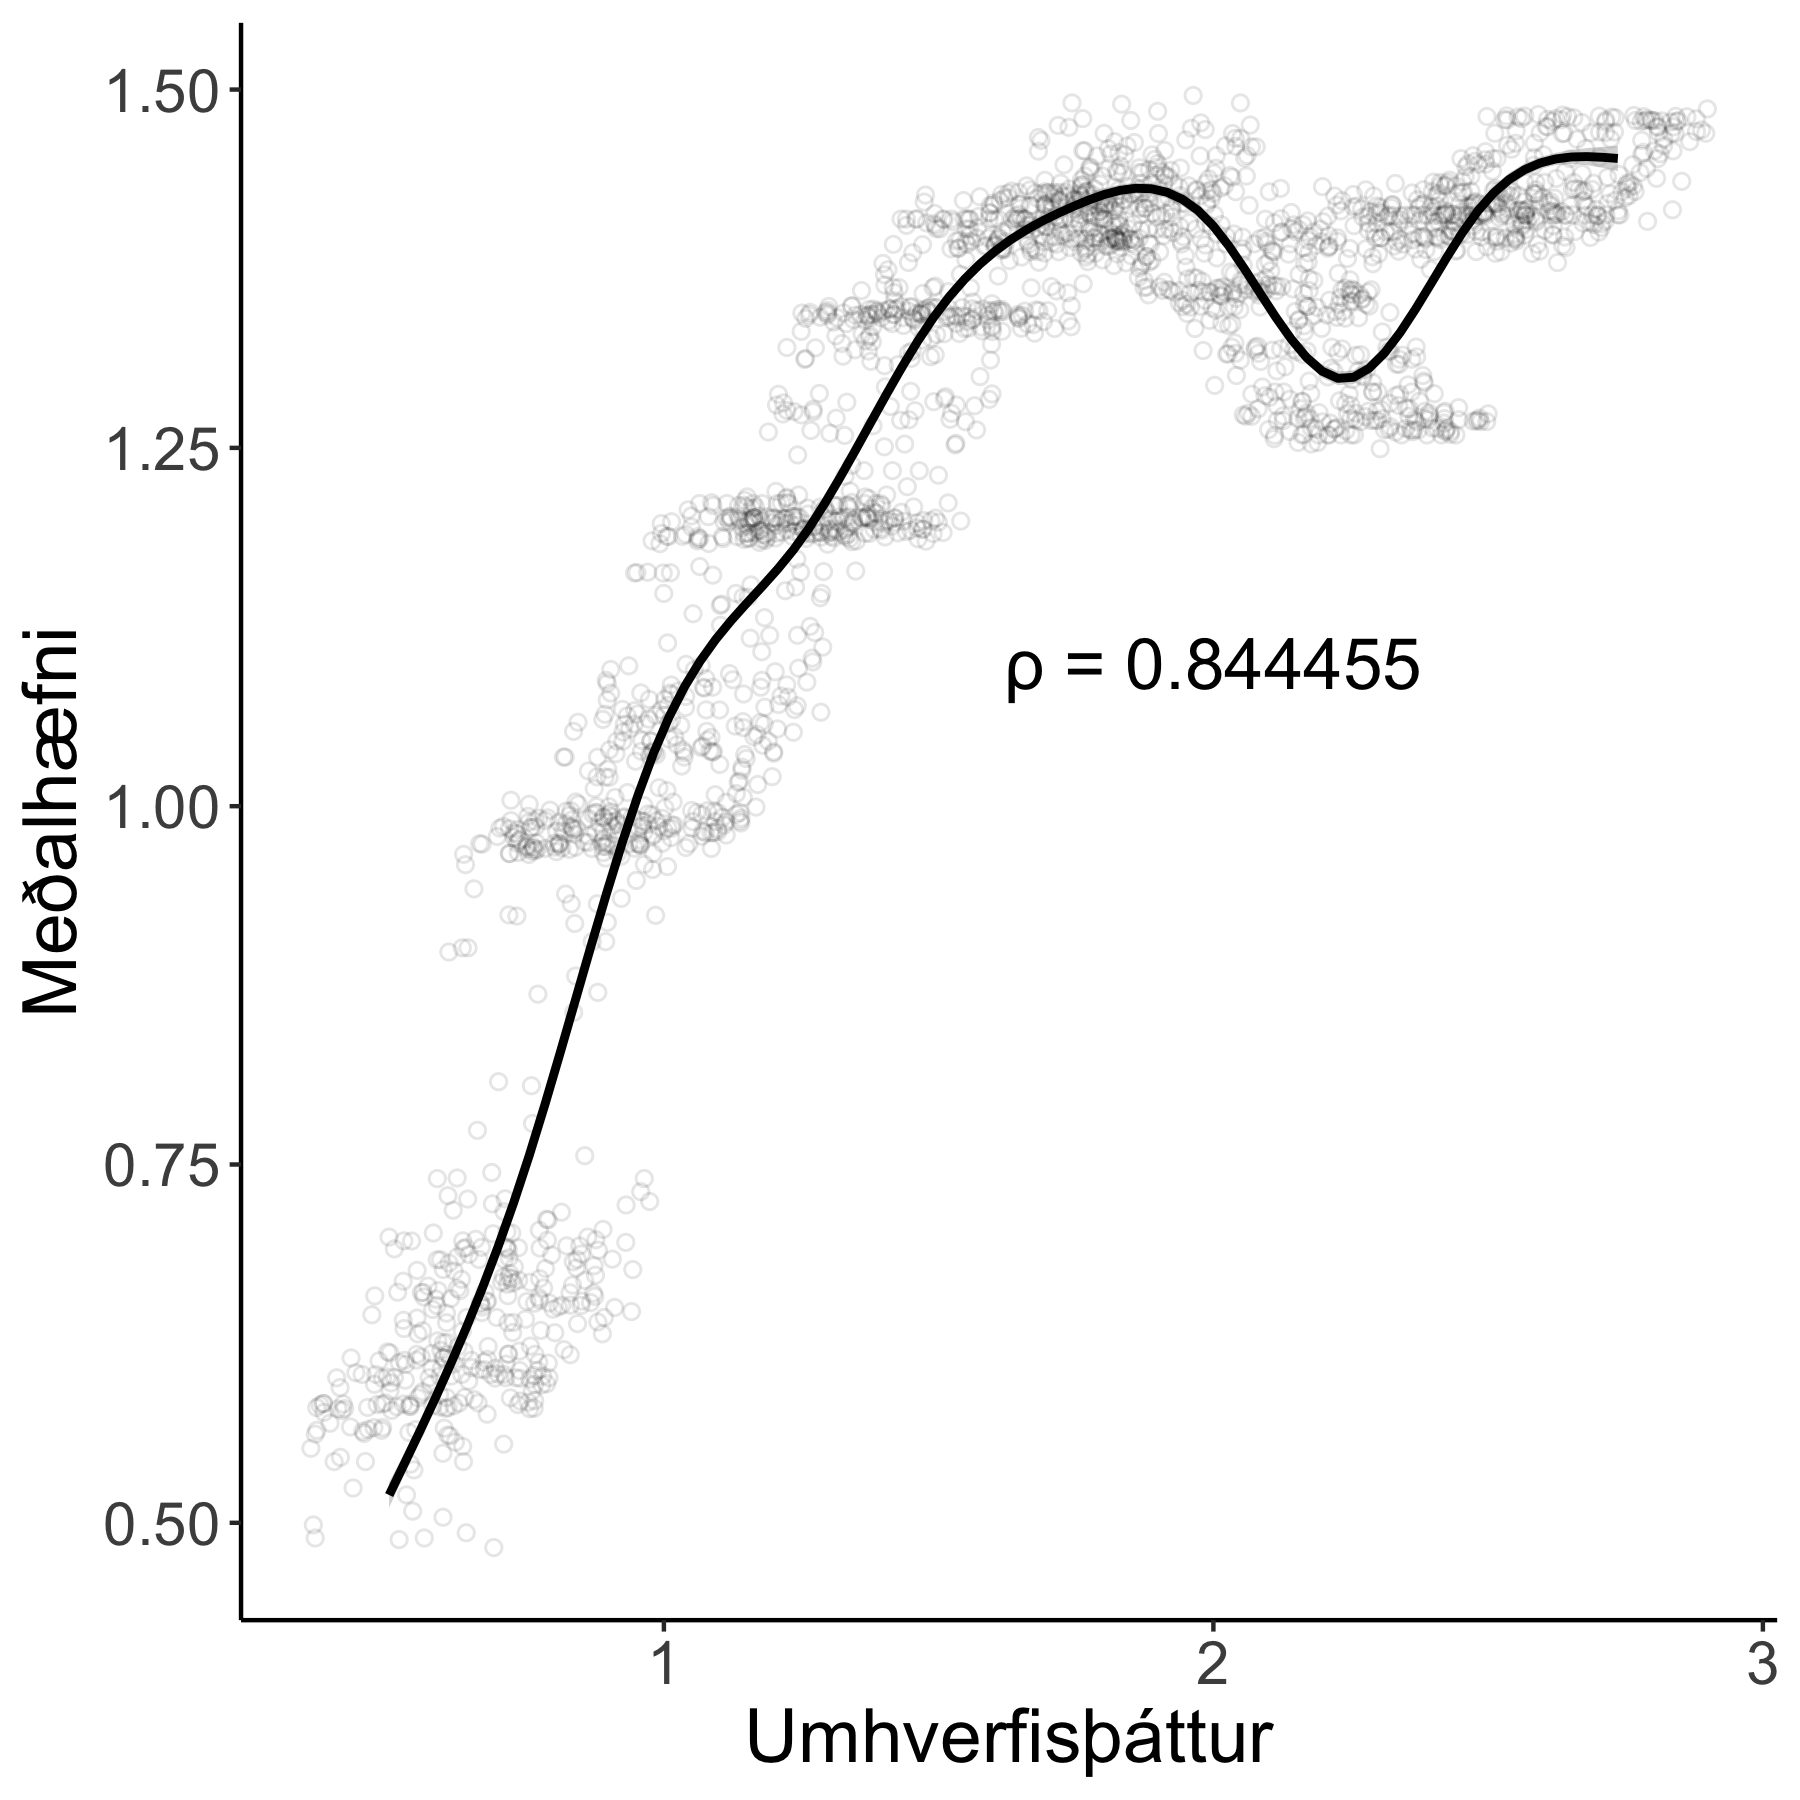
\includegraphics[width=\textwidth]{img/plotA.png}
        \caption*{\bfseries (A)}
    \end{subfigure}%
    \begin{subfigure}{.5\textwidth}
        \centering
        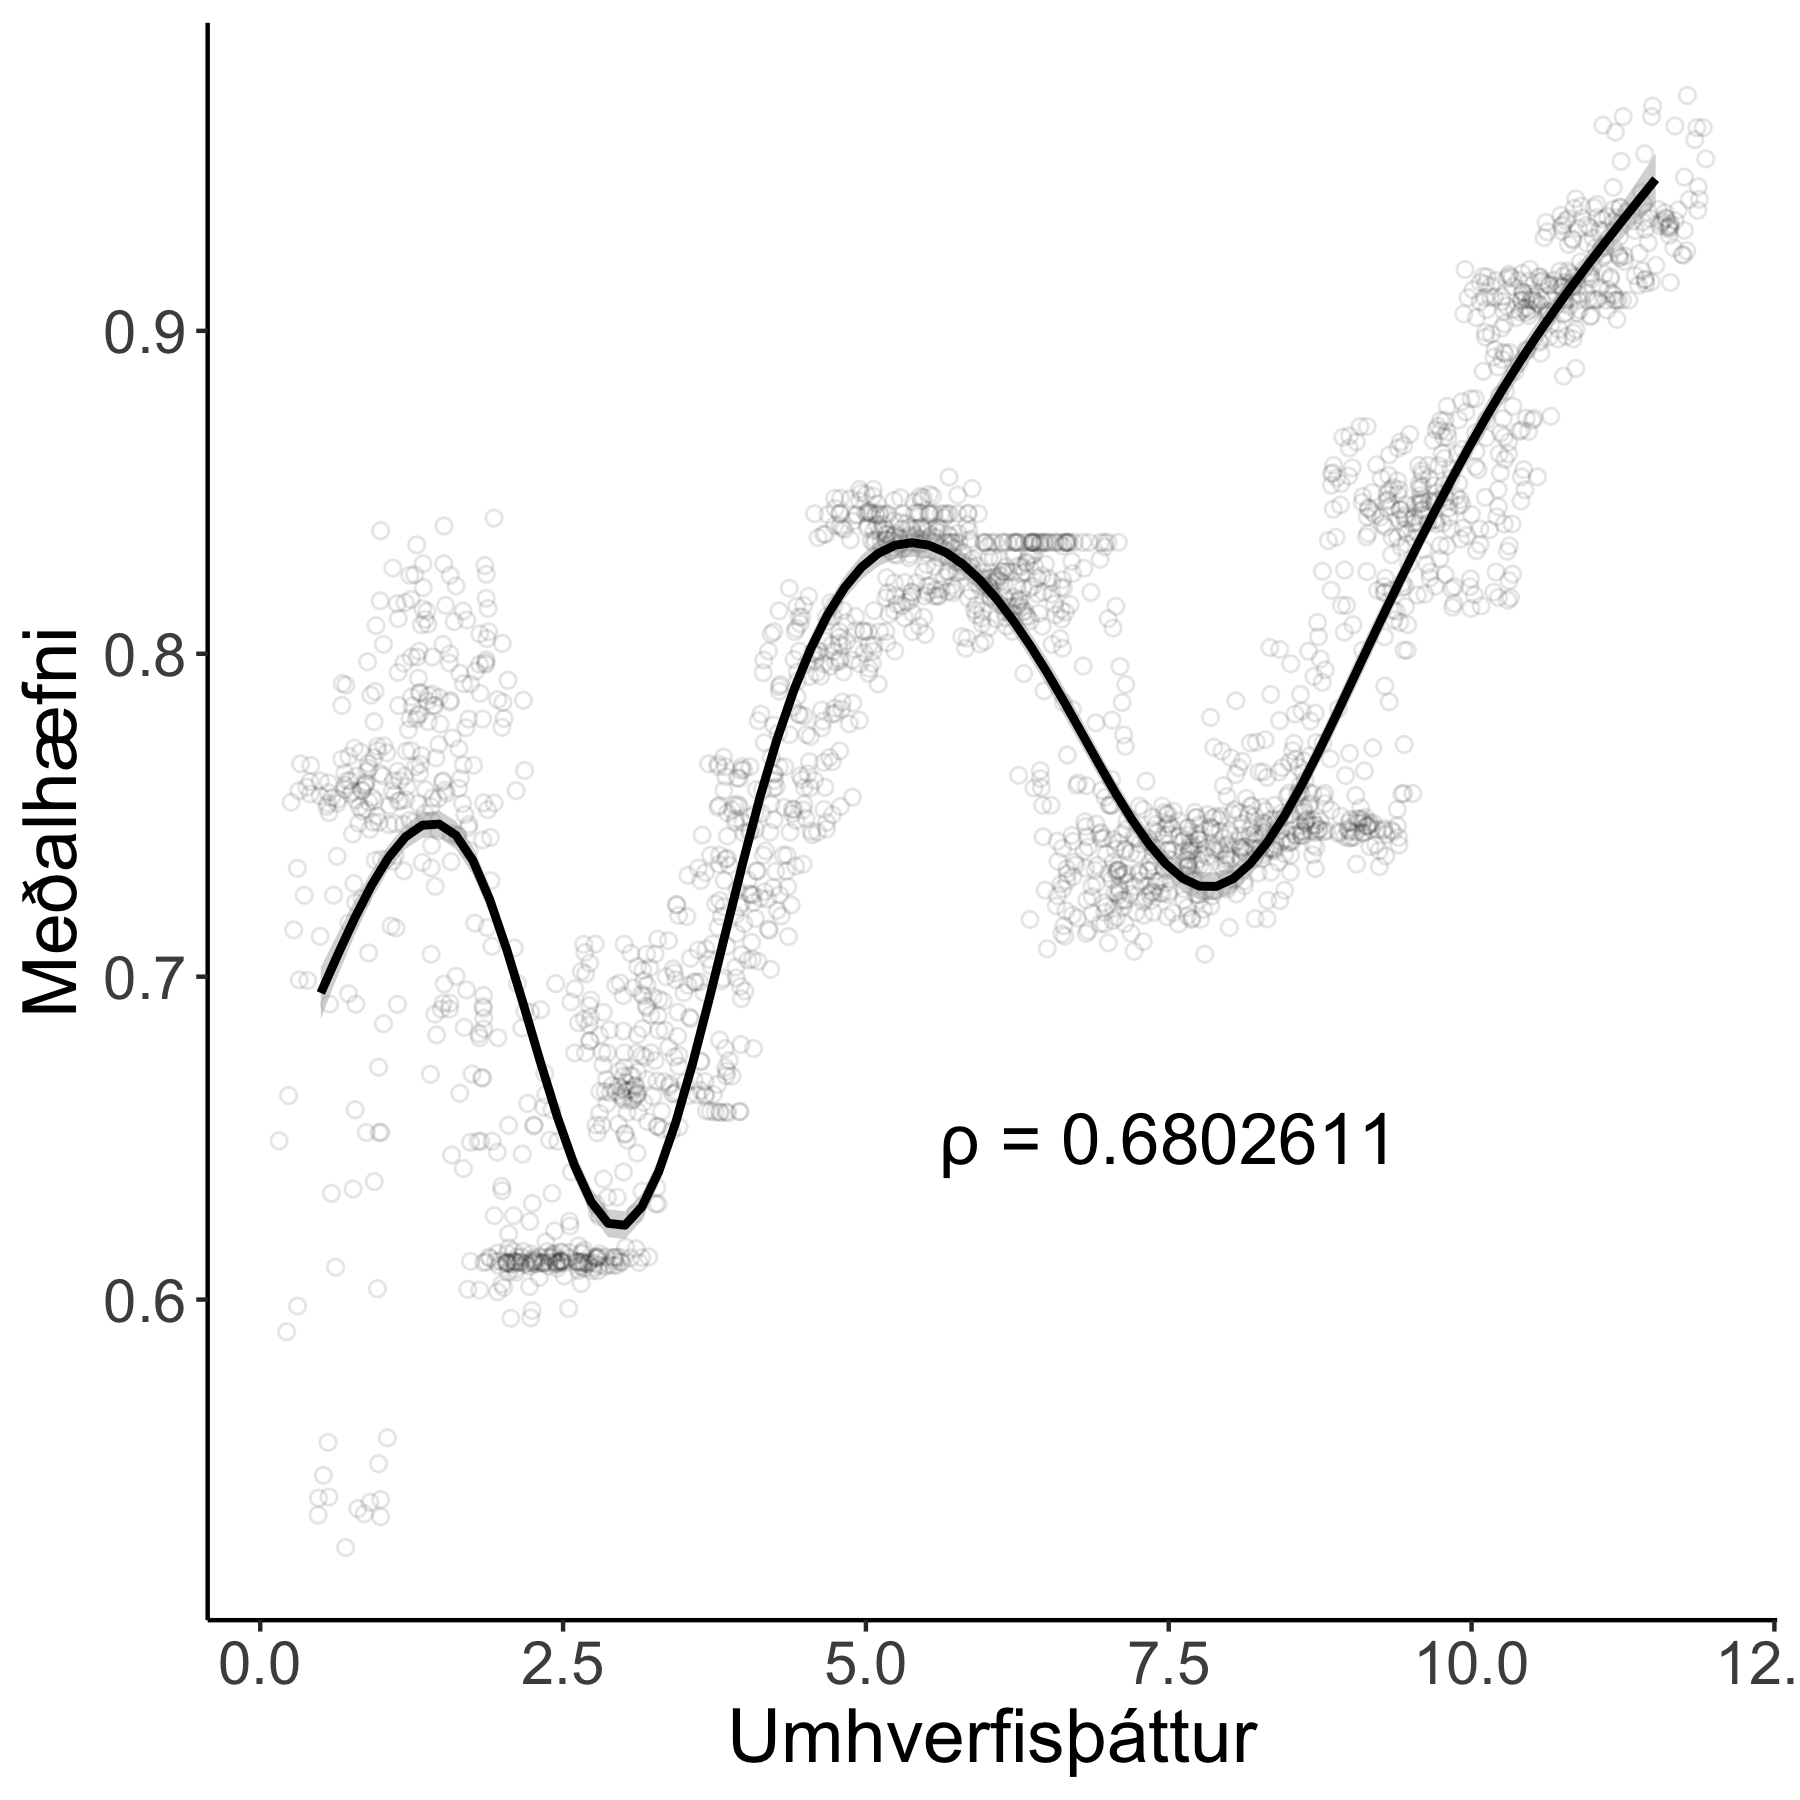
\includegraphics[width=\textwidth]{img/plotB.png}
        \caption*{\bfseries (B)}
    \end{subfigure} \\
    \begin{subfigure}{.5\textwidth}
        \centering
        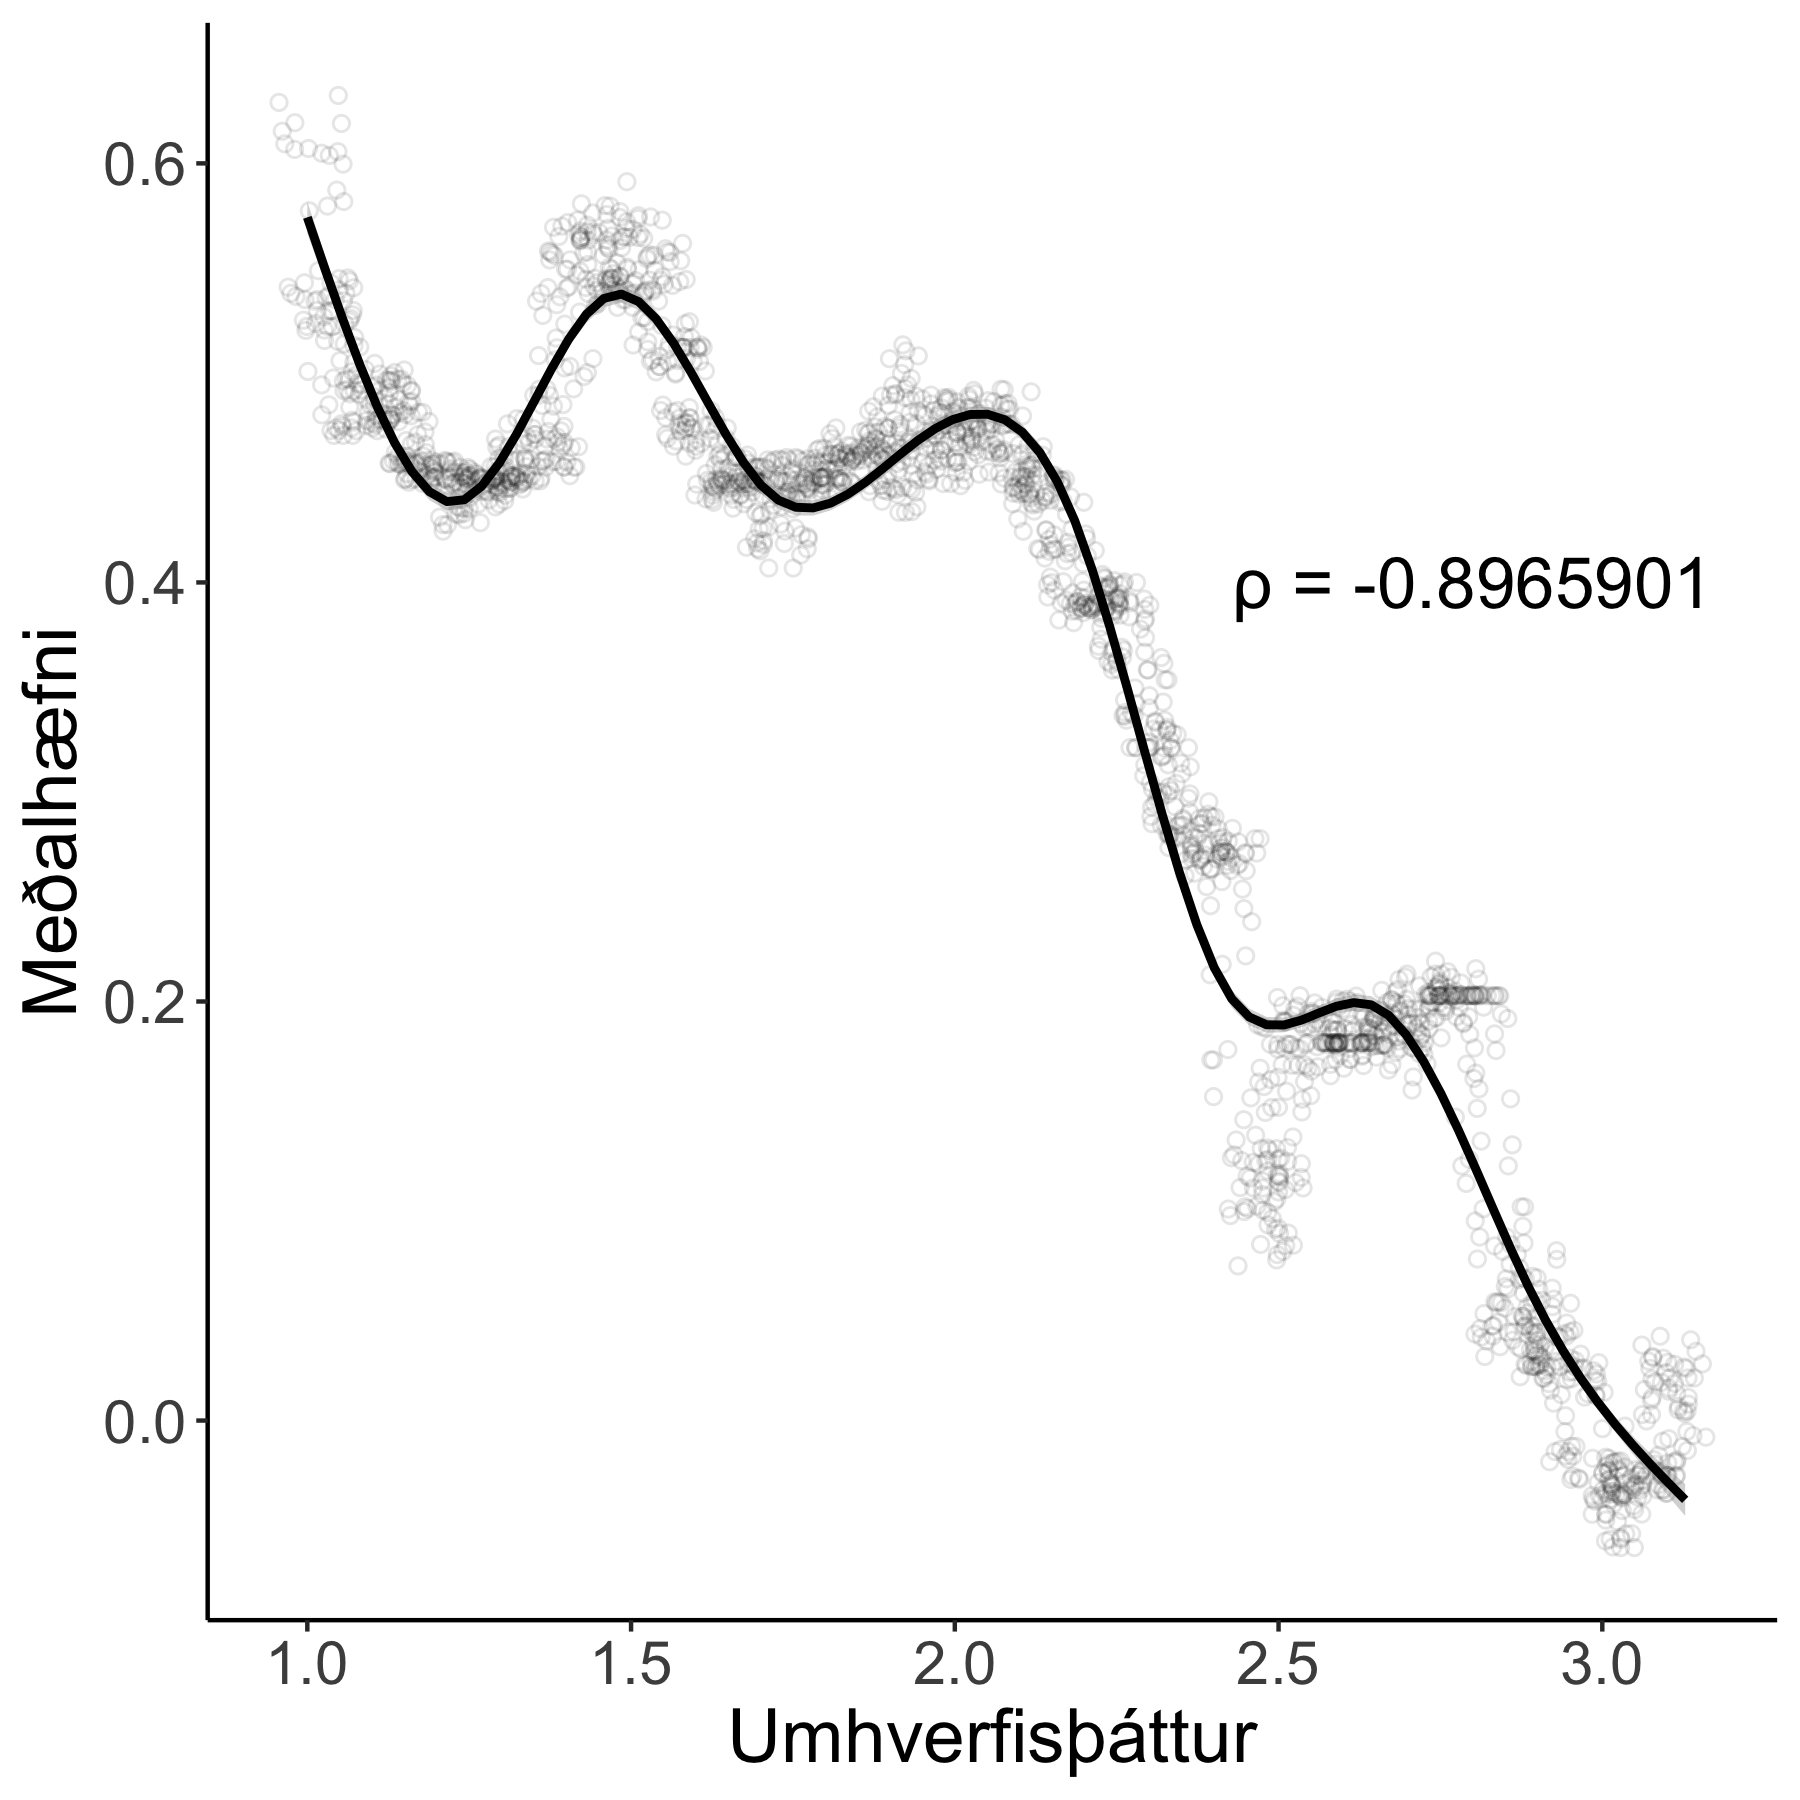
\includegraphics[width=\textwidth]{img/plotC.png}
        \caption*{\bfseries (C)}
    \end{subfigure}%
    \begin{subfigure}{.5\textwidth}
        \centering
        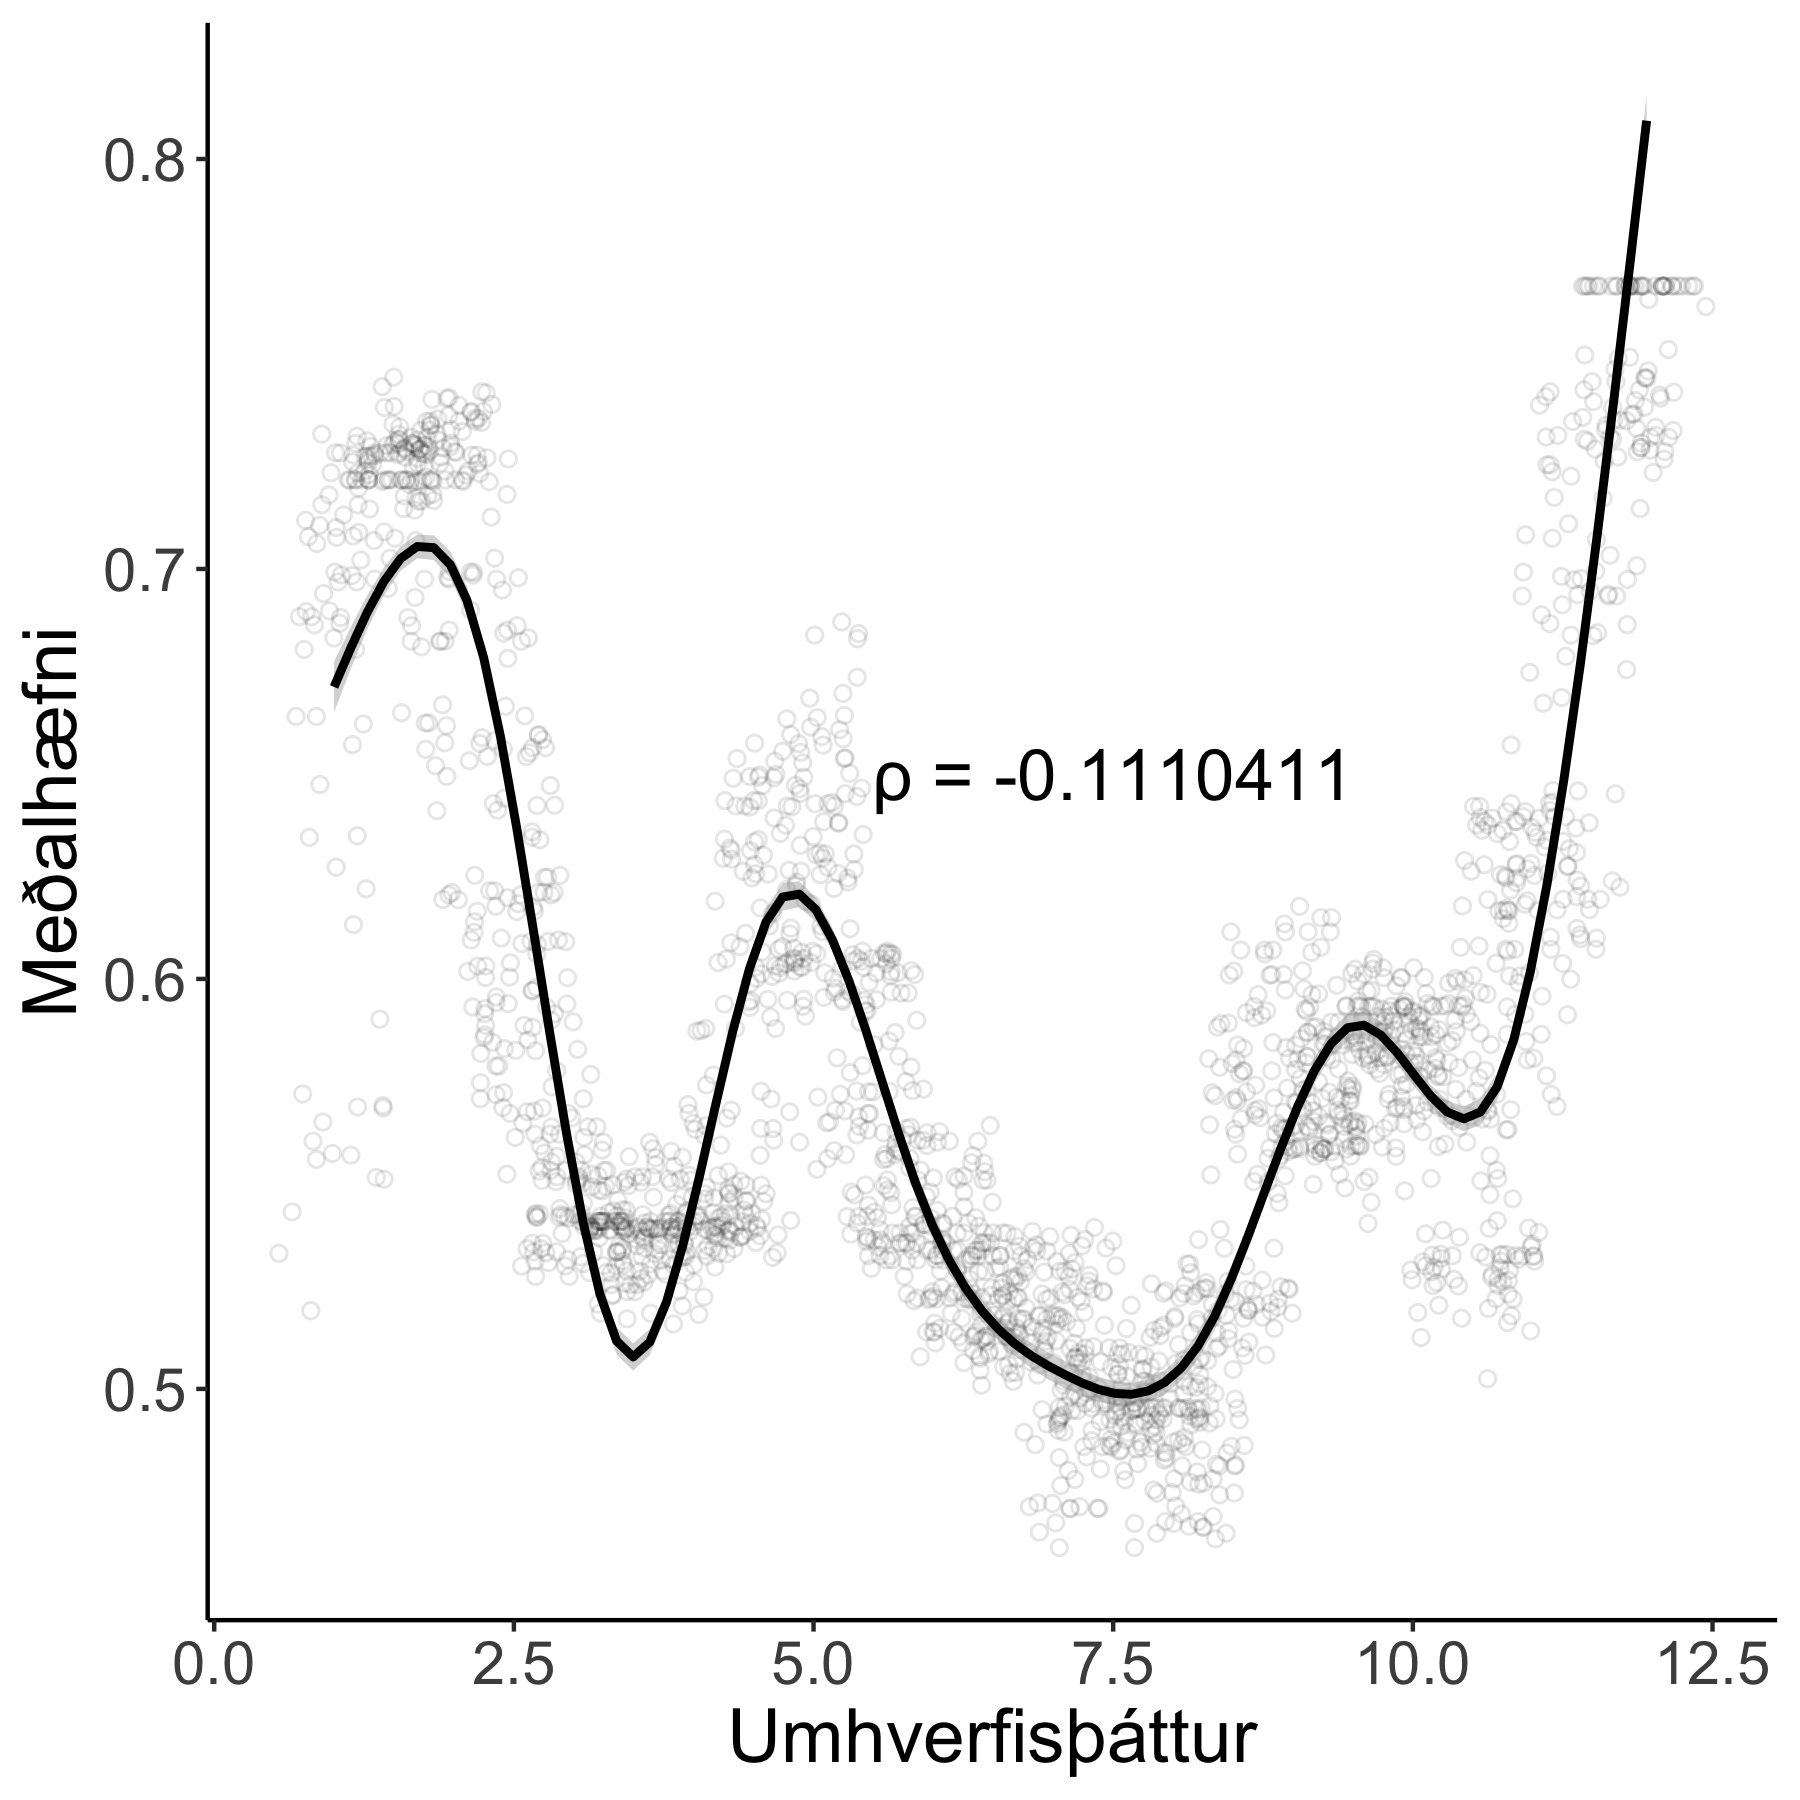
\includegraphics[width=\textwidth]{img/plotD.png}
        \caption*{\bfseries (D)}
    \end{subfigure}%
    \caption{Samband umhverfisþáttar og meðalhæfni}
\end{figure}

\end{document}